\documentclass[11pt,letterpaper]{article}
\usepackage[margin=1in]{geometry}
\usepackage{graphicx} % Required for inserting images
\usepackage{tikz}
\usepackage{amsthm,amsmath,amssymb}
\usepackage{algorithm}
\usepackage{algpseudocode}
\usepackage{xcolor}
\usepackage{soul}
\usepackage{enumitem}

% Theorems
\newtheorem{theorem}{Theorem}[section]
\newtheorem{corollary}[theorem]{Corollary}
\newtheorem{lemma}[theorem]{Lemma}
\newtheorem{claim}[theorem]{Claim}
\theoremstyle{definition}
\newtheorem{definition}[theorem]{Definition}
\newtheorem{remark}[theorem]{Remark}
\newtheorem{observation}[theorem]{Observation}

\newcommand{\reals}{\mathbb{R}}
\newcommand{\Span}{\mathrm{span}}
\newcommand{\coreq}{\mathrm{coreq}}

\newcommand{\calA}{\mathcal{A}}
\newcommand{\calB}{\mathcal{B}}
\newcommand{\calC}{\mathcal{C}}
\newcommand{\calD}{\mathcal{D}}
\newcommand{\calE}{\mathcal{E}}
\newcommand{\calF}{\mathcal{F}}
\newcommand{\calG}{\mathcal{G}}
\newcommand{\calH}{\mathcal{H}}
\newcommand{\calI}{\mathcal{I}}
\newcommand{\calJ}{\mathcal{J}}
\newcommand{\calK}{\mathcal{K}}
\newcommand{\calL}{\mathcal{L}}
\newcommand{\calM}{\mathcal{M}}
\newcommand{\calN}{\mathcal{N}}
\newcommand{\calO}{\mathcal{O}}
\newcommand{\calP}{\mathcal{P}}
\newcommand{\calQ}{\mathcal{Q}}
\newcommand{\calR}{\mathcal{R}}
\newcommand{\calS}{\mathcal{S}}
\newcommand{\calT}{\mathcal{T}}
\newcommand{\calU}{\mathcal{U}}
\newcommand{\calV}{\mathcal{V}}
\newcommand{\calW}{\mathcal{W}}
\newcommand{\calX}{\mathcal{X}}
\newcommand{\calY}{\mathcal{Y}}
\newcommand{\calZ}{\mathcal{Z}}

\newcommand{\bfa}{\mathbf{a}}
\newcommand{\bfb}{\mathbf{b}}
\newcommand{\bfc}{\mathbf{c}}
\newcommand{\bfd}{\mathbf{d}}
\newcommand{\bfe}{\mathbf{e}}
\newcommand{\bff}{\mathbf{f}}
\newcommand{\bfg}{\mathbf{g}}
\newcommand{\bfh}{\mathbf{h}}
\newcommand{\bfi}{\mathbf{i}}
\newcommand{\bfj}{\mathbf{j}}
\newcommand{\bfk}{\mathbf{k}}
\newcommand{\bfl}{\mathbf{l}}
\newcommand{\bfm}{\mathbf{m}}
\newcommand{\bfn}{\mathbf{n}}
\newcommand{\bfo}{\mathbf{o}}
\newcommand{\bfp}{\mathbf{p}}
\newcommand{\bfq}{\mathbf{q}}
\newcommand{\bfr}{\mathbf{r}}
\newcommand{\bfs}{\mathbf{s}}
\newcommand{\bft}{\mathbf{t}}
\newcommand{\bfu}{\mathbf{u}}
\newcommand{\bfv}{\mathbf{v}}
\newcommand{\bfw}{\mathbf{w}}
\newcommand{\bfx}{\mathbf{x}}
\newcommand{\bfy}{\mathbf{y}}
\newcommand{\bfz}{\mathbf{z}}

\newcommand{\cost}{\mathrm{COST}}
\newcommand{\ALG}{\mathrm{ALG}}
\newcommand{\OPT}{\mathrm{OPT}}
\newcommand{\Flow}{\textsc{Flow}}
\newcommand{\ouralg}{\textsc{LineTracker}}

\newcommand{\EE}{\mathbb{E}}

\newcommand{\interval}[1]{\lfloor #1 \rceil}
\newcommand{\off}{\mathrm{off}}
\newcommand{\on}{\mathrm{on}}
\newcommand{\org}{\mathrm{org}}
\newcommand{\rel}{\mathrm{rel}}
\newcommand{\dis}[1]{#1}
\newcommand{\new}{\mathrm{new}}

\newcommand{\solution}{\medskip\noindent\textbf{Solution.}\par\medskip}

\newcommand{\Var}{\mathrm{Var}}

\usepackage[hidelinks]{hyperref}
\usepackage{cleveref}


\title{47-836: Network Optimization II \\ Homework 3}
\author{Poon Tze-Yang}
\date{November 2026}


\begin{document}

\maketitle

Make your solutions concise and formal. Your goal is to convince me that you know the solutions. You should typeset your solutions in Latex. Please submit on Canvas. All of your algorithms should run in polynomial time and you should prove their correctness.

\begin{enumerate}[series=q]
\item Formulate the maximum flow problem as a linear program and derive its dual. Show that the dual corresponds to the minimum $s,t$-cut problem.
\end{enumerate}

\solution

Given a directed graph $G=(V,E)$ with edge capacities $\{c_e\}_{e \in E}$, we start with the flow-conservation primal: we have one variable for the flow on each edge, constrained to the capacity of the edge, and constrained so that flow is conserved at each vertex except for $s$ and $t$.
The objective is to maximize the flow out of $s$.
For simplicity, we assume that there are no edges into $s$.
\begin{align*}
    \max \sum_{e\in \delta^+(s)} f_e \\
    s.t. \sum_{e\in\delta^+(v)} f_e - \sum_{e\in\delta^-(v)} f_e &= 0,\quad \forall v \in V\setminus\{s,t\} \\
    0 \leq f_e &\leq c_e,\quad \forall e \in E.
\end{align*}
Next, we show that this is equivalent to the following path formulation: with one variable for each $s,t$-path, constrained to the capacity of each edge, and constrained so that the flow on each edge is equal to the sum of the flows on all paths that use that edge.
Let $P$ be the set of all $s,t$-paths in $G$.
\begin{align*}
    \max \sum_{p\in P} g_p \\
    s.t. \sum_{p\in P: e\in p} g_p &\leq c_e,\quad \forall e \in E \\
    g_p &\geq 0,\quad \forall p \in P.
\end{align*}
We show equivalence by showing that any feasible solution for one formulation can be converted to a feasible solution for the other.
Given a feasible solution $\{g_p\}_{p\in P}$ for the path formulation, we can construct a feasible solution $\{f_e\}_{e\in E}$ for the flow-conservation formulation by setting $f_e = \sum_{p\in P: e\in p} g_p$.
This is feasible because the capacity constraints are already satisfied, and the flow is conserved on the non-endpoint vertices of each path, so it is also conserved over the sum of paths.

Given a feasible solution $\{f_e\}_{e\in E}$ for the flow-conservation formulation, we can construct a feasible solution $\{g_p\}_{p\in P}$ for the path formulation by decomposing the flow into paths.
We can do this by repeatedly finding shortest $s,t$-paths from $s$ to $t$, sending as much flow as possible along that path.
We are guaranteed that we can always find a path because flow is conserved at each intermediate vertex and there are no edges into $s$, so we eventually reach $t$.
We repeat this in the residual graph until there are no more $s,t$-paths, which means that the sum of the flows along all paths in our constructed solution is equal to the flow out of $s$ in the original solution.
Capacity constraints are satisfied because we only send flow along edges of the residual graph.

Now, we take the dual of the path formulation.
We have one variable for each edge, and one constraint for each $s,t$-path.
\begin{align*}
    \min \sum_{e\in E} c_e y_e \\
    s.t. \sum_{e\in p} y_e &\geq 1,\quad \forall p \in P \\
    y_e &\geq 0,\quad \forall e \in E.
\end{align*}
Note that every cut corresponds to a feasible dual solution: every cut has at least one edge on every $s,t$-path.
By Menger's theorem, the value of the max flow is equal to the value of the min cut, so an optimal solution to the dual corresponds to a minimum cut.



\begin{enumerate}[resume=q]
\item The \emph{MAX-CUT} problem is defined as follows. Given a weighted undirected graph
\[
G = (V, E, w),
\]
find a cut
\[
(S, V \setminus S)
\]
that maximizes the total weight of edges crossing the cut, i.e.,
\[
\text{maximize}\ \sum_{\substack{(u,v) \in E \\ u \in S,\, v \notin S}} w(u,v).
\]
\begin{enumerate}
\item Give a randomized $\frac{1}{2}$-approximation in expectation for this problem.
\end{enumerate}
\end{enumerate}

\solution
Algorithm: For each vertex $v\in V$, assign $v$ to $S$ with probability $\frac{1}{2}$ independently.

Analysis: For each edge, the probability that it is in the cut is $\frac{1}{2}$, so the expected weight of the cut is $\frac{1}{2}\sum w(e)$.
An upper bound on the weight of the max cut is $\sum w(e)$, so the expected weight of the cut is at least $\frac{1}{2}$ of the max cut.


\begin{enumerate}[resume=q]
\item Let $G = (V, E)$ be a directed graph representing a flow network and say that there are integer capacities on the edges. Let $s$ and $t$ be two unique nodes denoting the source and sink. A $s,t$ cut is a set of vertices $S \subset V$ where $s \in S$. The capacity of the cut is $c(\delta^+(S)) = \sum_{e \in \delta^+(S)} c(e)$. We are interested in minimum capacity $s,t$ cuts. Call a set $S$ minimal if no. proper subset of $S$ is also a min-cut.
\begin{enumerate}
\item Prove that there is a \emph{unique} minimal min-cut.
\item Give an algorithm to compute the minimal min-cut
\end{enumerate}
\end{enumerate}

\solution

(a): A standard fact is that the directed cut function is submodular: for any two sets $A, B \subseteq V$,
\[
c(\delta^+(A)) + c(\delta^+(B)) \geq c(\delta^+(A \cap B)) + c(\delta^+(A \cup B)).   
\] 
(Proof is basically the same as the proof that the undirected cut function is submodular, which we did in q3 of hw1.)

If $A$ and $B$ are both min-cuts, then the left-hand side is equal to $2\lambda$, where $\lambda$ is the value of the min-cut.
The right-hand side is at least $2\lambda$, so we have equality throughout and $A\cap B$ is a min-cut.
This shows that the intersection of any two min-cuts is a min-cut, so the intersection of all min-cuts is a min-cut.
This intersection is unique and minimal, so there is a unique minimal min-cut.

(b): To compute the minimal min-cut, first, we compute a max flow.
Then, we compute the residual graph and find the set of vertices reachable from $s$ in the residual graph.
By Menger's theorem, this is a min-cut.
This is also a minimal min-cut, since any proper subset of this set has residual edges crossing the cut, so it is not a min-cut.
By the above argument, this is the unique minimal min-cut.

\begin{enumerate}[resume=q]
\item Let $G = (V, E)$ be a undirected simple graph. Let $T \subseteq V$ be a set of terminals. We refer to $V \setminus T$ as the non-terminals. For $u, v \in T$ define the \emph{element} connectivity as $\kappa'(u, v)$ as the maximum number of $u-v$ paths that are disjoint in the non-terminals and edges of $G$. Note paths can share terminals. See the figure.
\begin{enumerate}
\item Given $G = (V, E)$, $T \subseteq V$ and $u, v \in T$ describe an efficient algorithm to compute $\kappa'(u, v)$.
\item Prove that for $u, v, w \in T$, $\kappa'(u, v) \geq \min\{\kappa'(u, w), \kappa'(v, w)\}$
\end{enumerate}

\begin{figure}[ht]
\centering
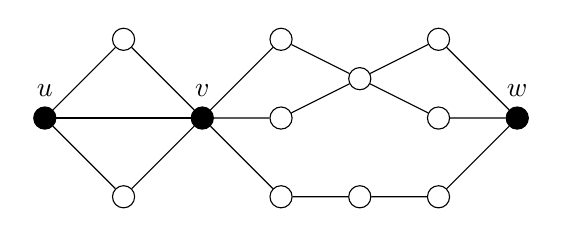
\begin{tikzpicture}[
    terminal/.style={circle, draw, fill=black, inner sep=0pt, minimum size=8pt},
    nonterminal/.style={circle, draw, fill=white, inner sep=0pt, minimum size=8pt}]
% terminals
\node[terminal, label=above:$u$] (u) at (0,0) {};
\node[terminal, label=above:$v$] (v) at (2,0) {};
\node[terminal, label=above:$w$] (w) at (6,0) {};

% non-terminals
\node[nonterminal] (a1) at (1,1) {};
\node[nonterminal] (a2) at (1,-1) {};
\node[nonterminal] (b1) at (3,1) {};
\node[nonterminal] (b2) at (3,0) {};
\node[nonterminal] (m) at (4,0.5) {};
\node[nonterminal] (c1) at (5,1) {};
\node[nonterminal] (c2) at (5,0) {};
\node[nonterminal] (d1) at (3,-1) {};
\node[nonterminal] (d2) at (4,-1) {};
\node[nonterminal] (d3) at (5,-1) {};

% edges
\draw (u) -- (v);
\draw (u) -- (a1) -- (v);
\draw (u) -- (a2) -- (v);
\draw (v) -- (b1) -- (m) -- (c1) -- (w);
\draw (v) -- (b2) -- (m) -- (c2) -- (w);
\draw (v) -- (d1) -- (d2) -- (d3) -- (w);
\end{tikzpicture}
\caption{In the graph above $\kappa'(u,v) = 3$ and $\kappa'(u,w) = \kappa'(v,w) = 2$.}
\label{fig:element-connectivity}
\end{figure}
\end{enumerate}

\solution
(a): We will reduce the problem to a max flow problem on a directed graph.
First, we replace all edges $uv$ with the following gadget: we add two new vertices $x,x'$ and replace the edge $uv$ with the arcs $u\to x$, $v\to x$, $x\to x'$, $x' \to u$, $x'\to v$.
Thus, any path that uses the edge $uv$ must use the arc $x\to x'$, so only one unit of flow can use this edge.
Next, we replace each non-terminal vertex $v$ with the following gadget: we add two new vertices $v_{in}, v_{out}$ and replace all arcs $u\to v$ with $u\to v_{in}$ and all arcs $v\to w$ with $v_{out}\to w$, and add the arc $v_{in}\to v_{out}$.
Thus, any path that uses the vertex $v$ must now use the arc $v_{in}\to v_{out}$, so only one unit of flow can use this vertex.
Then, the maximum flow from $u$ to $v$ in this directed graph is equal to $\kappa'(u,v)$, since a max flow corresponds to an element-disjoint flow in the original graph, and vice versa.

(b): Using the directed graph $G'$ constructed above, $\kappa'(u,w)$ is the size of some maximum edge-disjoint flow $F_{uw}$ from $u$ to $w$ in $G'$.
Similarly, we have an element-disjoint flow of size $\kappa'(v,w)$ from $v$ to $w$ in the original graph. This is equal to a $w$ to $v$ element-disjoint flow in the original graph, which corresponds to a $w$ to $v$ flow $F_{wv}$ in $G'$.


Suppose $\kappa'(u,v) = \min\{\kappa'(u,w),\kappa'(v,w)\}$ (the other case is symmetric), so we can define a flow $F'_{wv}$ of size $\kappa'(u,v)$ by removing some flow from $F_{wv}$.
Combining $F = F_{uw}\cup F'_{wv}$ gives a flow from $u$ to $v$ of value $\kappa'(u,v)$, where some arcs are reused.
We deal with reused edges by shortcutting:
suppose there exists an arc $e=xy$ used by both $u,w$-path $P_{uw}\in F_{uw}$ and $w,v$-path $P_{wv}\in F'_{wv}$.
Then we have a directed cycle in $F$ starting from $e$, following $P_{uw}$ to $w$, then $P_{wv}$ back to $x$.
Removing this cycle from $F$ preserves the flow value and eliminates the reused arc.
Repeating this process until no arcs are reused gives an edge-disjoint flow from $u$ to $v$ of value $\kappa'(u,w)$, so we can lower bound the max flow from $u$ to $v$ by $\kappa'(u,v)\geq\kappa'(u,w)$.
Each edge-disjoint flow in $G'$ defines an element-disjoint flow in $G$ of the same size, so this lower bounds the size of the max element-disjoint flow in $G$ from $u$ to $v$ by the same bound.




\end{document}
